\documentclass{article}%
\usepackage[T1]{fontenc}%
\usepackage[utf8]{inputenc}%
\usepackage{lmodern}%
\usepackage{textcomp}%
\usepackage{lastpage}%
\usepackage[head=40pt,margin=0.5in,bottom=0.6in]{geometry}%
\usepackage{graphicx}%
%
\title{\textbf{Estudiantes del Pedagógico de Caracas exigieron condiciones dignas}}%
\author{El Nacional}%
\date{04/12/2018}%
%
\begin{document}%
\normalsize%
\maketitle%
\textbf{URL: }%
http://www.el{-}nacional.com/noticias/sociedad/estudiantes{-}del{-}pedagogico{-}caracas{-}exigieron{-}condiciones{-}dignas\_262032\newline%
%
\textbf{Periodico: }%
EN, %
ID: %
262032, %
Seccion: %
Sociedad\newline%
%
\textbf{Palabras Claves: }%
NO\_TIENE\newline%
%
\textbf{Derecho: }%
2.2, %
Otros Derechos: %
, %
Sub Derechos: %
2.2.1\newline%
%
\textbf{EP: }%
SI\newline%
\newline%
%
\textbf{\textit{Las personas cerraron la vía con palos para impedir el paso de los vehículos}}%
\newline%
\newline%
%
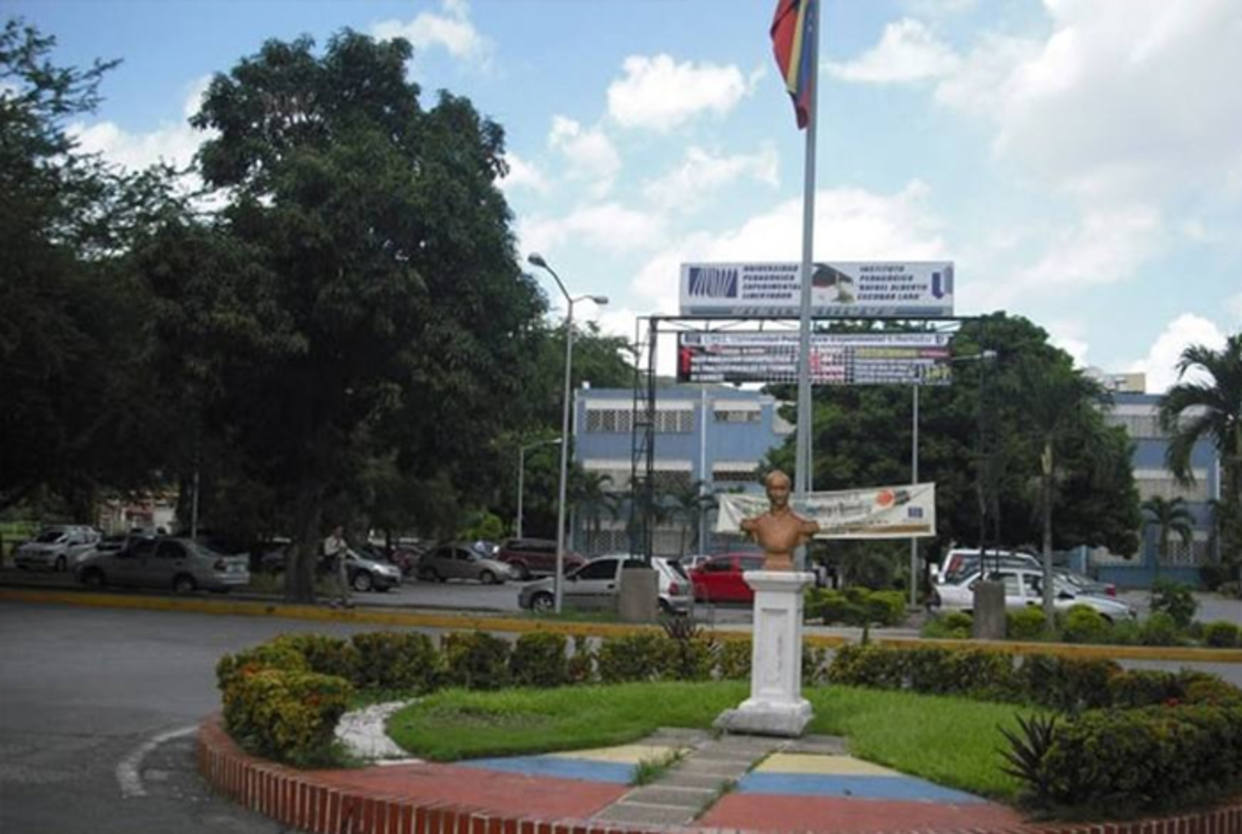
\includegraphics[width=300px]{65.jpg}%
\newline%
%
Los estudiantes de la Universidad Pedagógica Experimental Libertador protestaron ayer para exigir condiciones dignas en el proceso educativo.%
\newline%
%
Los jóvenes cerraron la avenida Páez, en El Paraíso, en horas de la mañana. Atravesaron palos, lo que ocasionó largas colas de vehículos. La comunidad tuvo que armarse de paciencia y soportar el reclamo. La Guardia Nacional Bolivariana llegó al sitio e intentó impedir la tranca, por lo cual se vivieron momentos de tensión.%
\newline%
%
La protesta se extendió hasta pasadas las horas del mediodía. Los alumnos tocaron tambores para exigir la atención de las autoridades.%
\newline%
%
“No tenemos agua, comedor, becas, profesores, biblioteca. Exigimos atención”, se leía en una de las pancartas que mostraba una de las estudiantes.%
\newline%
%
Los jóvenes se quejan de que los espacios del centro de estudios están sucios, en condiciones deplorables. Además, dicen que su período académico está en riesgo por la falta de docentes.%
\newline%
%
“Estamos cansados de pedirle al Estado que nos apoye”, indicó uno de los muchachos presentes en la manifestación. “Nosotros queremos que nos escuchen y atiendan nuestra petición”, afirmó.%
\newline%
%
Indicó que tienen asignada una beca de cuatro bolívares soberanos, lo que considera insuficiente para poder afrontar los costos universitarios ante el incremento constante de los precios. “¿Qué podemos hacer con eso?”, preguntó.%
\newline%
%
\end{document}